%% USPSC-Codificação64b/66b.tex

% ----------------------------------------------------------
% Codificação 64b/66b 
% ----------------------------------------------------------
\chapter[A codificação 64b/66b]{A codificação 64b/66b} \label{codificacao64b66b}

Este tipo de codificação garante transições suficientes para realizar a recuperação de \textit{clock} no lado do receptor, além de preservar a probabilidade de detectar somente um ou múltiplos erros nos bits durante a transmissão. Os dois bits de sincronização adicionados no código permitem alinhar o fluxo dos blocos de bits no receptor.

\section{Convenções de Notação}

A codificação codifica um byte de dados ou um byte de caracteres de controle em um bloco. Os blocos que contém caracteres de controle também contém um campo com o tipo do bloco. Os octetos de dados são rotulados de D0 até D7. Caracteres de controle, tirando os O, S, e T, são rotulados de C0 até C7. Os caracteres de controle para definição de ordem são rotulados como O0 e O4 desde que seja válido o primeiro octeto do XGMII. Os caracteres de controle para o início são rotulados como S0 e S4 para a mesma condição do octeto do XGMII. Os caracteres de controle para o fim são rotulados como T0 e T7.

Duas transferências consecutivas de XMGII fornece oito caracteres que são codificados em um bloco da transmissão de 66-bits. O subíndice dos rótulos acima indica a posição dos caracteres na transferência dos 8 caracteres do XMGII.

O conteúdo do campo do tipo de bloco, os octetos de dados e os caracteres de controle são exibidos em valores hexadecimais. O bit menos significativo (LSB) do valor hexadecimal representa o primeiro a ser transmitido. Por exemplo, enviando o campo do tipo de bloco Ox1E na verdade em binário oque é enviado é “01111000”. Os bits de um bloco transmitido ou recebido são rotulados como TxB<65:0> e RxB<65:0>, respectivamente, em que TxB<0> e RxB<0> representam o primeiro bit transmitido. O valor do cabeçalho de sincronização é mostrado como valor binário. Os valores binários são mostrados com o primeiro bit transmitido (LSB) na esquerda.

\section{Estrutura do Bloco}

Os blocos consistem em 66 bits. Os primeiros dois bits de um bloco são os cabeçalhos de sincronização. Os blocos podem ser dado, controle ou os dois ao mesmo tempo. Os bits de sincronismo são definidos como “01” para blocos de dados e “10” para blocos de controle. Portanto, sempre há uma transição entre os dois primeiros bits do bloco para obter uma sincronização do bloco. O restante do bloco contém o dado útil. Somente o dado útil passa pelo \textit{scrambler}, diferentemente dos bits de sincronismo uma vez que são somente adicionados ao dado de saída do \textit{scrambler} sem passar pelo mesmo.

Blocos de dados contém 8 bytes diferentemente dos blocos de controle os quais começam com um bloco de tipo de 8 bits, indicando o formato do restante do bloco. Para blocos de controle que possuem caracteres de começo e de término no meio dos 64 bits, sendo definidos pelo \textit{control tipe field}. Outros caracteres de controles são codificados em 7 bits ou 4 bits representando o código de controle “O”.

O formato dos blocos é como ilustrado na \autoref{table64b66b}. Na coluna \textit{Input Data} mostra de forma abreviada o formato dos 8 bytes usados para criar o bloco de 66 bits. Os campos com retângulos finos representam um único bit, sendo preenchidos com o bit “0” e ignorados pelo receptor.

\begin{figure}[H]
	\caption{\label{table64b66b}Formato dos blocos da codificação 64b/66b}
	\centering
	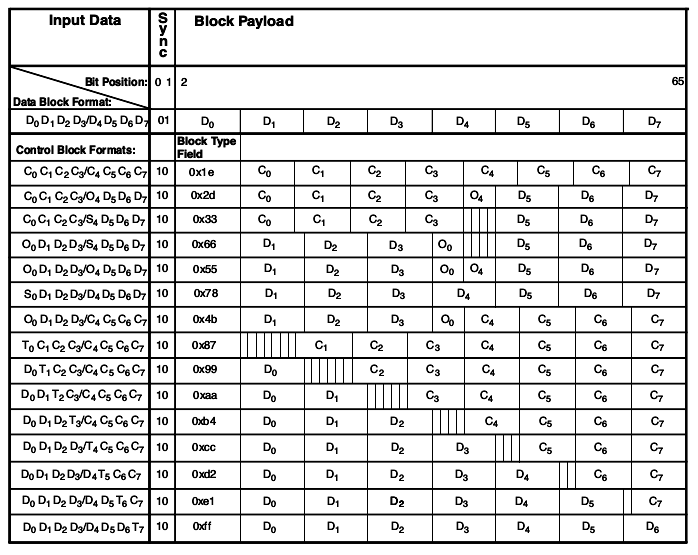
\includegraphics[scale=0.9]{tabela64b66b.png}
	\begin{center}
		Fonte: Elaborado pelo Autor
	\end{center}	
\end{figure}

Os bits e as posições dos campos são mostrados com o bit menos significativo na esquerda. Por exemplo, o \textit{block type field} “0x1E” é enviado como 01111000 representando os bits de 2 até 9 do bloco de 66 bits. O bit menos significativo de cada campo está numerado na menor posição do bloco. 

Todos os outros valores não utilizados para o \textit{control tipe field} são reservados. Estes valores foram escolhidos para possuírem uma distância de Hamming de 4 bits. O único valor, em hexadecimal, não utilizado o qual mantém esta regra é 0x00.

\section{Códigos de Controle}

O mesmo conjunto de caracteres de controle é suportado pelo XMGII e pelo 10GBASE-R PCS. Os valores correspondentes para os caracteres de controle são denominados como códigos de controle. O XMGII codifica um caracter para um octeto (dado de 8bits). O 10GBASE-R PCS codifica implicitamente os caracteres de controle de \textit{start} e de \textit{terminate} pelo \textit{control tipe field}. O 10BASE-R PCS codifica o código de controle de ordenamento (\textit{ordered\_set control codes}) usando uma combinação de \textit{block type field} e um código de ordenamento de 4 bits (\textit{4-bit O code}) para cada código \textit{ordered\_set}. O 10GBASE-R PCS codifica todos os outros caracteres de controle para um código de 7 bits (\textit{7-bits C code}). 
Os caracteres de controle e o seu mapeamento para o 10GBASE-R PCS está descrito na tabela da \autoref{comando64b66b}. Qualquer ou valor que não está presente na tabela da \autoref{comando64b66b} não deve ser transmitido e deverá ser tratado como erro.

\begin{figure}[H]
	\caption{\label{comando64b66b}Tabela dos códigos de controle da codificação 64b/66b.}
	\centering
	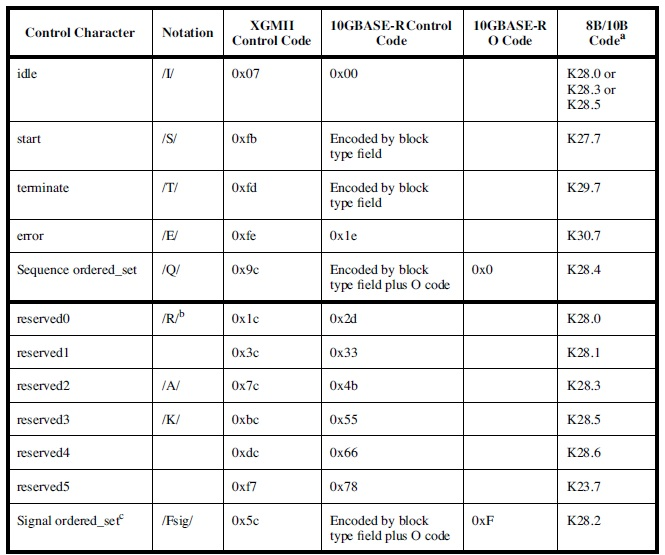
\includegraphics[scale=0.9]{command64b66b.png}
	\begin{center}
		Fonte: Elaborado pelo Autor
	\end{center}	
\end{figure}

A coluna do 8b/10b code está representada de forma informativa. A utilização dos códigos de controle da codificação 8b/10b está descrito na secção 48 da especificação do IEEE 802.3ae \cite{IEEstandard}. Os códigos /A/, /K/ e /R/ são usados nas interfaces XAUI para sinais de espera. 

\subsection{Idle (/I/)}

Este comando de controle refere-se quando se deseja inserir uma espera no sistema, bem como para adaptar o sistema aos ciclos de clock. Os caracteres de controle (/I/) são transmitidos quando um sinal de espera é recebido do XGMII. Inserção ou retirada de caracteres /I/ devem ocorrer em grupos de 4 bits. Ao adicionar estes caracteres, deve-se seguir o controle de espera ou os ordered\_sets. Os caracteres de controle /I/ não devem serem inseridos enquanto está recebendo algum dado. Quando 

\subsection{Start (/S/)}

Este caracter de controle é comumente usado somente para os blocos onde um início pode acontecer. O \textit{start control character} (/S/) indica o início de um pacote. Este delimitador é válido somente no primeiro bloco dos 64 bits do XGMII (TXD<0:7> e RXD <0:7>). A recepção de um \textit{start control character} em qualquer outro octeto do TxD indica-se um erro na transmissão. Os valores do \textit{block type field} implicitamente codifica um /S/ como quinto ou o primeiro bloco de 8 bits do dado de 64 bits. 

\subsection{Teminate (/T/)}

O \textit{terminate control character } (/T/) indica o final do pacote. Como os pacotes possuem comprimentos variados, o caracter de controle (/T/) pode ocorrer em qualquer octeto da interface XGMII. A localização do comando é codificada implicitamente pelo \textit{block type field}. Um término de pacote é válido quando um bloco contendo um controle /T/ é seguido por um bloco que não contém um controle /T/.

\subsection{Ordered\_set (/O/)}

O caracter controle \textit{ordered\_set} pode indicar dois tipos de comando: uma sequência que o caracter de controle possui ou um sinal de ordenamento. Necessitando denominar a sequência dos caracteres de controle para o \textit{ordered\_sets}, deverá ser usado o controle /Q/ descrito na tabela da \autoref{comando64b66b}. O caracter /O/ somente é válido no primeiro octeto do XGMII, caso é recebido em qualquer outro bloco de 8 bits indica um erro. O próprio \textit{block type field} codifica implicitamente um comando /O/ no primeiro ou no quinto bloco de 8 bits do dado de 64 bits, desta forma qualquer outra posição que o comando /O/ estiver significa um erro. O \textit{block type field} já codifica implicitamente o controle /O/ no primeiro ou no quinto bloco de 8 bits. O 4-bit O codifica o caracter /O/ específico para o \textit{ordered\_set}.

A sequência dos \textit{ordered\_sets} pode ser deletada pelo PCS para se adaptar entre os ciclos de \textit{clock}. Esta operação só pode ser realizada quando duas sequências consecutivas do comando forem recebidas e somente uma destas é deletada. Para a compensação de \textit{clock}, exclusivamente comandos \textit{idle} podem serem inseridos. Sinais \textit{ordered\_sets} não podem serem excluídos para compensação do \textit{clock}.

\subsection{Error (/E/)}

O comando /E/ é enviado sempre que o mesmo ou um bloco inválido é recebido. O comando de erro permite as camadas físicas como o XGXS e o PCS propagar sinais de erros. Um esclarecimento maior sobre os sinais pode ser obtido na cláusula 49.2.13.2.3 da especificação do IEEE 802.3ae \cite{IEEstandard}. 


\section{Ordered\_sets}

Os sinais de comando \textit{ordered\_sets} são usado para ampliar a capacidade de enviar sinais de controle e estado pelo link, como falha remota e estado da falha remota local. \textit{Ordered\_sets} são caracteres de controle seguidos de 3 caracteres de dados e sempre começam no primeiro bloco de 8 bits do XGMII. O \textit{10 Gigabit Ethernet} usa um tipo de \textit{ordered\_set} descrito na cláusula 46.3.4 do padrão IEEE 802.3ae \cite{IEEstandard}. A sequência de caracteres de controle \textit{ordered\_set} é denotado /Q/. Um código adicional de controle, o sinal \textit{ordered\_sets}, está reservado e começa com outro código de controle. O campo de 4 bits (O) codifica os códigos de controle. Veja mais na tabela da \autoref{comando64b66b}. 

\section{Blocos válidos e inválidos} 

Um bloco é inválido quando:

\begin{itemize}
	\item Os bits de sincronismo do bloco de 66bits forem "00" ou "11"
	\item O \textit{block type field} conter um valor reservado descrito na tabela da \autoref{comando64b66b}.
	\item Qualquer caracter de controle não possuir alguns dos valores descritos na tabela da \autoref{comando64b66b}.
	\item Qualquer caracter de ordenamento (\textit{ordered\_sets}) /O/ que não esteja na tabela da \autoref{comando64b66b}.
	\item O bloco de 64 bits não possuir algum dos formatos descritos na tabela da \autoref{table64b66b}.
\end{itemize}

\section{Scrambler} \label{scramb:64b66b}

Na maioria dos sistemas de comunicações o propósito de um circuito scrambler é balancear o máximo possível as transições no dado a ser transmitido, evitando níveis lógicos repetidos por muito tempo. Desta forma, o circuito scrambler possibilita uma recuperação de \textit{clock} do lado do receptor, além de fornecer um espectro de potência mais disperso diminuindo as interferências de rádio e o \textit{crosstalk}, uma vez que a potência não está concentrada em uma única frequência.

O princípio básico de funcionamento de um circuito scrambler são os \textit{linear feedback shift register} (LFSR). Um \textit{shif register} de comprimento "n" consiste em n-flipflops interconectados, possuindo o estado binário desta célula de memória com índice (i) transferida para uma célula com índice (i +1) quando um sinal de \textit{clock} é aplicado em todas estas células. Cada flip-flop é visto como um estágio do registro e a informação binária do último estágio é sempre acessível fisicamente.

Para a implementação da codificão 64b/66b foi utilizado o \textit{scrambler} e o \textit{descrambler} definidos nas cláusulas 49.2.6 e 49.2.10 do padrão IEEE 802.3ae \cite{IEEstandard}.O sistema do \textit{scrambler} e do \textit{descrambler} é ilustrado na \autoref{des_scrambler_IEEE}.

\begin{figure}[H]
	\caption{\label{des_scrambler_IEEE} Esquema do \textit{scrambler} e do \textit{descrambler} descrito no padrão IEEE 802.3ae.}
	\centering
	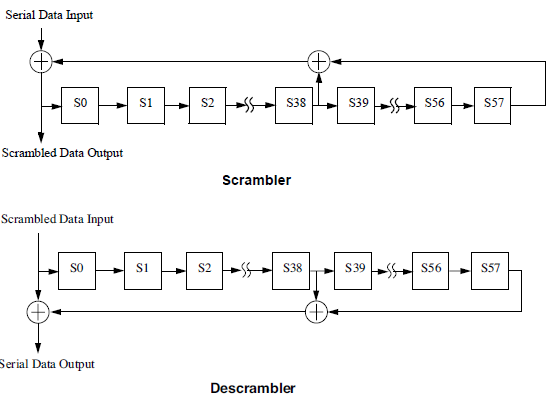
\includegraphics[scale=1.0]{des_scrambler_IEEE.png}
	\begin{center}
		Fonte: Elaborado pelo Autor
	\end{center}	
\end{figure}

Os 64 bits são inseridos no sistema, já os 2 bits de sincronismo são anexados com a saída do \textit{scrambler} sem passar pelo mesmo. Para o \textit{descrambler} o procedimento é o mesmo que no \textit{scrambler}. Nos dois sistemas é usado o seguinte polinômio:

$$ G(x) = x^{58} + x^{39} + 1 $$

Este polinômio é primitivo gerando uma sequência de $2^{58} - 1 = 288230376151711743$ números, sendo muito difícil de a sequência ser descoberta por alguém. 

Em qualquer transmissão de dados é possível ocorrer ruídos, desta forma o \textit{descrambler} da \autoref{des_scrambler_IEEE} ao receber os dados errôneos, além de multiplicar erros como descrito no \autoref{scrambler_multi}, pode carregar estes para um novo dado de entrada. Na \autoref{errosDesc} é descrito as possibilidades de carregar o erro ocorrido no dado atual para um novo dado.

\begin{figure}[H]
	\caption{\label{errosDesc} Possibilidades de carregamento de erros no Descrambler.}
	\centering
	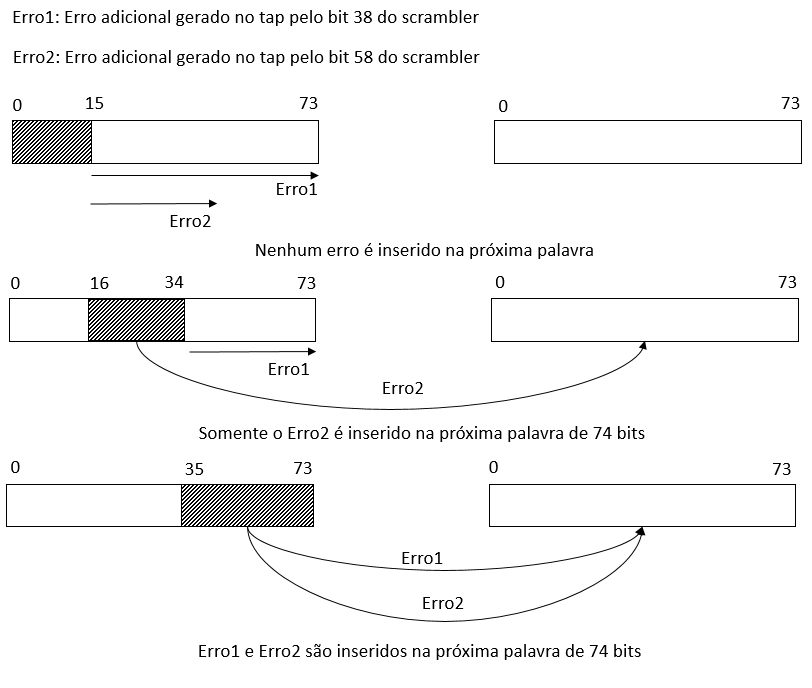
\includegraphics[scale=0.7]{erroPositionDescrambler.png}
	\begin{center}
		Fonte: Elaborado pelo Autor
	\end{center}	
\end{figure}

Observa-se que desta forma um único bit errôneo pode gerar erros nos novos dados que possivelmente estão corretos.

\section{CRC-8 bits} \label{crc8}

Como visto, o erro de um bit pode se propagar para um erro de três bits depois de passar pelo \textit{descrambler} além de poder ser carregado para um novo dado de entrada. Por isso, é necessário detectá-los com um sistema adequado. A teoria para o entendimento do funcionamento do CRC implementado no sistema e a escolha do polinômio adequado pode ser vista na seção \autoref{crc:teoria}. A tabela com os polinômios ideais para cada distância de hamming pode ser encontrada em \cite{Philip2018}.  

Portanto, implementou-se um CRC de 8 bits com o polinômio $0x83= [1 0 0 0 0 0 1 1] = x^{8} + x^{2} + x + 1$ e com distância de Hamming igual a 4, como descrito na tabela presente em \cite{CRCTable2018}. Fatorando este polinômio obtêm-se $(x + 1)(x^{7} + x^{6} + x^{5} + x^{4} + x^{3} + x^{2} + 1)$ que ao ser comparado com a teoria da \autoref{poli:gerador} pode-se obter algumas características do sistema. Portanto, pela teoria descrita observa-se que o polinômio pode detectar qualquer tipo de erro. Os erros de rajada podem serem detectados pois o polinômio não possui um fator $x$ presente, a não ser na condição descrita na \autoref{poli:gerador}. Já os erros ímpares podem serem detectados pois o polinômio possui um fator $(x + 1)$ ao ser expandido. Os erros duplos ou pares não podem serem detectados uma vez que o polinômio é múltiplo do fator $x^{i}(1 + x^{j − i})$. Os erros simples também são detectáveis pois o polinômio possui mais que dois termos.

O CRC que implementa o polinômio descrito está ilustrado na \autoref{crc_8b_bits}. Observa-se que primeiramente o dado é inserido, permanecendo a chave na posição mais escura. Posteriormente a chave move-se para a posição mais clara e o resto é obtido dos registradores.

\begin{figure}[H]
	\caption{\label{crc_8b_bits} Esquemático do CRC-8 Bits implementado na codificação 64b/66b.}
	\centering
	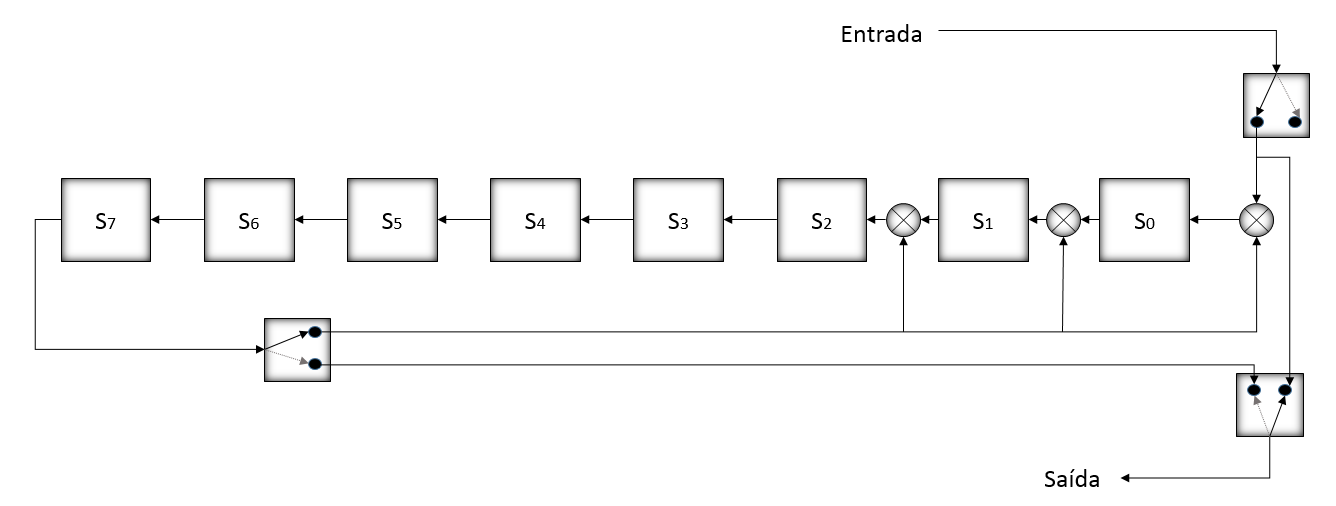
\includegraphics[scale=0.45]{crc_8_bits.png}
	\begin{center}
		Fonte: Elaborado pelo Autor
	\end{center}	
\end{figure}

Desta maneira, o CRC pode detectar erros de até 3 bits em com comprimento até 119 bits, possuindo um polinômio primitivo e capaz de detectar erros de número ímpar de bits \cite{Tridib2004}. 